\chapter{Introduction}

\section{Correlation Function}
\begin{figure}[tbp]
	\centering
	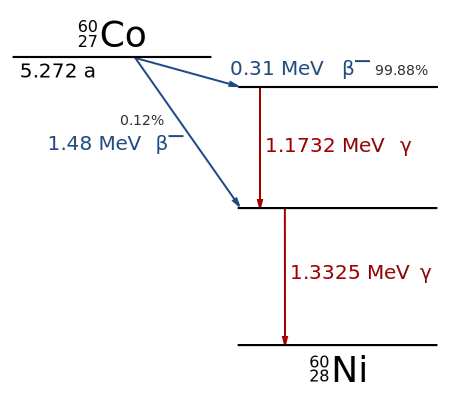
\includegraphics[width=.4\textwidth]{./img/co60_decay.pdf}
	\caption*{Source: \url{commons.wikimedia.org/wiki/File:Cobalt-60_Decay_Scheme.svg}}
	\caption[The decay cascade of \ce{^{60}Co}]{\textbf{The decay cascade of \ce{^{60}Co}} After decaying from a 5+ spin state to a 4+ spin state of \ce{^{60}Ni} by beta decay with a probability of \num{99.88}\%, two gamma rays of energies \SI{1.17}{\MeV} and \SI{1.33}{\MeV} are emitted, each inhibting a spin of 2+.}
	\label{fig:co60_cascade}
\end{figure}
When a nucleus in an excited state emits two gamma rays in a cascade, as shown in \autoref{fig:co60_cascade}, the spatial angular distribution of the second photon with respect to the first photon's direction of travel is anisotropic.
In particular, by detecting two rays of a cascade simultaneously, the equal population of states is removed, resulting in an anisotropy of the second ray's angular distribution.
The relative probability of the gamma ray's emission at an angle $\theta$ relative to the first photon is denoted as $W(\theta)$.
Normalizing this differential cross-section at $\theta=\SI{90}{\degree}$ yields the correlation function

\begin{equation*}
	K(\theta) = 1 + \sum_{k}^{k_\text{max}}a_{2k}\cdot\cos^{2k}{\theta}.
\end{equation*}

The series terminates at $k_\text{max}=\min(I, L_1, L_2)=2$, where $I, L_1, L_2$ denote the nuclear spin after the first gamma emission and the angular momenta of both gamma rays respectively.
This results in the correlation function

\begin{equation}\label{eq:corr_func}
	K(\theta) = 1 + a_2\cos^{2}{\theta} + a_4\cos^{4}{\theta},
\end{equation}
while only pure multipole orders (quadrupoles) are assumed.

By measuring coincidence counts for varying angles, coefficients $a_2$ and $a_4$ can be determined.
Defining the quantities
\begin{align}
	A&=\frac{N_\text{C}(\SI{135}{\degree})}{N_\text{C}(\SI{90}{\degree})} \label{eq:A}\\
	B&=\frac{N_\text{C}(\SI{180}{\degree})}{N_\text{C}(\SI{90}{\degree})}, \label{eq:B}
\end{align}
where $N_\text{C}(\theta)$ are coincidence event counts, simplifies the equations for $a_2$ and $a_4$ to
\begin{align}
	a_4 &= 2\cdot(1+B-2A) \label{eq:a4}\\
	a_2 &= 4A-B-3. \label{eq:a2}
\end{align}

The deviation of a correlation function from an isotropic angular distribution is called \textbf{anisotropy}
\begin{equation}\label{eq:aniso}
	An=\frac{K(180)-K(90)}{K(90)}=B-1.
\end{equation}

\section{Detectors}\label{sec:detectors}
To detect and measure the energy of gamma rays, which allows to discriminate between secondary and tertiary gamma radiation (for example caused by Compton scattering with the detector coating), two \ce{NaI}-scintillators doped with \ce{Th} are used.
Sodium iodide is an inorganic scintillator crystal, giving the advantage of most of the gamma rays being observed through the photoelectric effect.
Coupled to these scintillator crystals are two photomultiplier stages that output a voltage spike proportional to the incoming gamma ray's energy.
The output is digitized for later analysis.

\section{Resolution Time}
The timeframe, in which two individual events on each detector channel can be interpreted as a coincidence, is called the \textbf{resolution time (of a coincidence)}.
Utilizing the relation
\begin{equation}\label{eq:res_time}
	\tau_\text{res}=\frac{N_\text{F}}{N_1\cdot N_2}\cdot T,
\end{equation}
the resolution time can be computed, where used quantities are denoted as follows:
\begin{itemize}
	\item $N_\text{F}$ - false coincidences event count
	\item $N_{1/2}$ - number of events on channel 1/2
	\item $T$ length of measurement.
\end{itemize}
